\chapter{System design and implementation}
This chapter discusses the architecture and implementation of the KubeFold project.


\section{KubeFold Platform Concept}
KubeFold is software that operates on the Kubernetes platform in Operator manner.
The project consists of the following components:
\begin{itemize}
    \item Kubernetes Operator - a component that manages business logic.
    It ensures proper deployment and management of pods responsible for downloading protein databases and performing computations.
    This component is described in detail in section~\ref{subsec:component-operator}.
    \item Downloader Component - controls the process of downloading and decompressing protein databases.
    A detailed description can be found in section~\ref{subsec:component-downloader}.
    \item Manager Component - handles additional operations around computations such as artifact delivery or sending notifications.
    It is described in section~\ref{subsec:component-manager}.
\end{itemize}

Additionally, KubeFold introduces two Custom Resource Definitions (CRDs).
The first is the \texttt{ProteinDatabase} resource.
It represents a single installation of a protein database in the cluster.
An example resource code is shown in listing~\ref{lst:protein_database}.
In the resource specification, users can select which databases should be installed.
Furthermore, they can specify which StorageClass should be used for the volume storing the data.
This enables specifying a class that corresponds to the Lustre file system (described in section~\ref{subsec:lustre-volumes}).
In the example code, the class named \texttt{fsx-sc} is specified, which connects to AWS FSx for Lustre volumes (see~\ref{subsec:amazon-fsx-for-lustre}).
From the user's perspective, this resource can be managed using \texttt{kubectl} as shown in figure~\ref{fig:proteindatabase_terminal}.

\begin{lstlisting}[language=yaml,caption={Example \texttt{ProteinDatabase} resource definition},label={lst:protein_database}]
apiVersion: data.kubefold.io/v1
kind: ProteinDatabase
metadata:
  name: proteindatabase-sample
spec:
  datasets:
    bfd: true
    mgyclusters: true
    nt: true
    pdb: true
    pdbseqreq: true
    rfam: true
    rnacentral: true
    uniref90: true
    uniprot: true
  volume:
    storageClassName: fsx-sc
\end{lstlisting}

\begin{figure}[htbp]
    \centering
    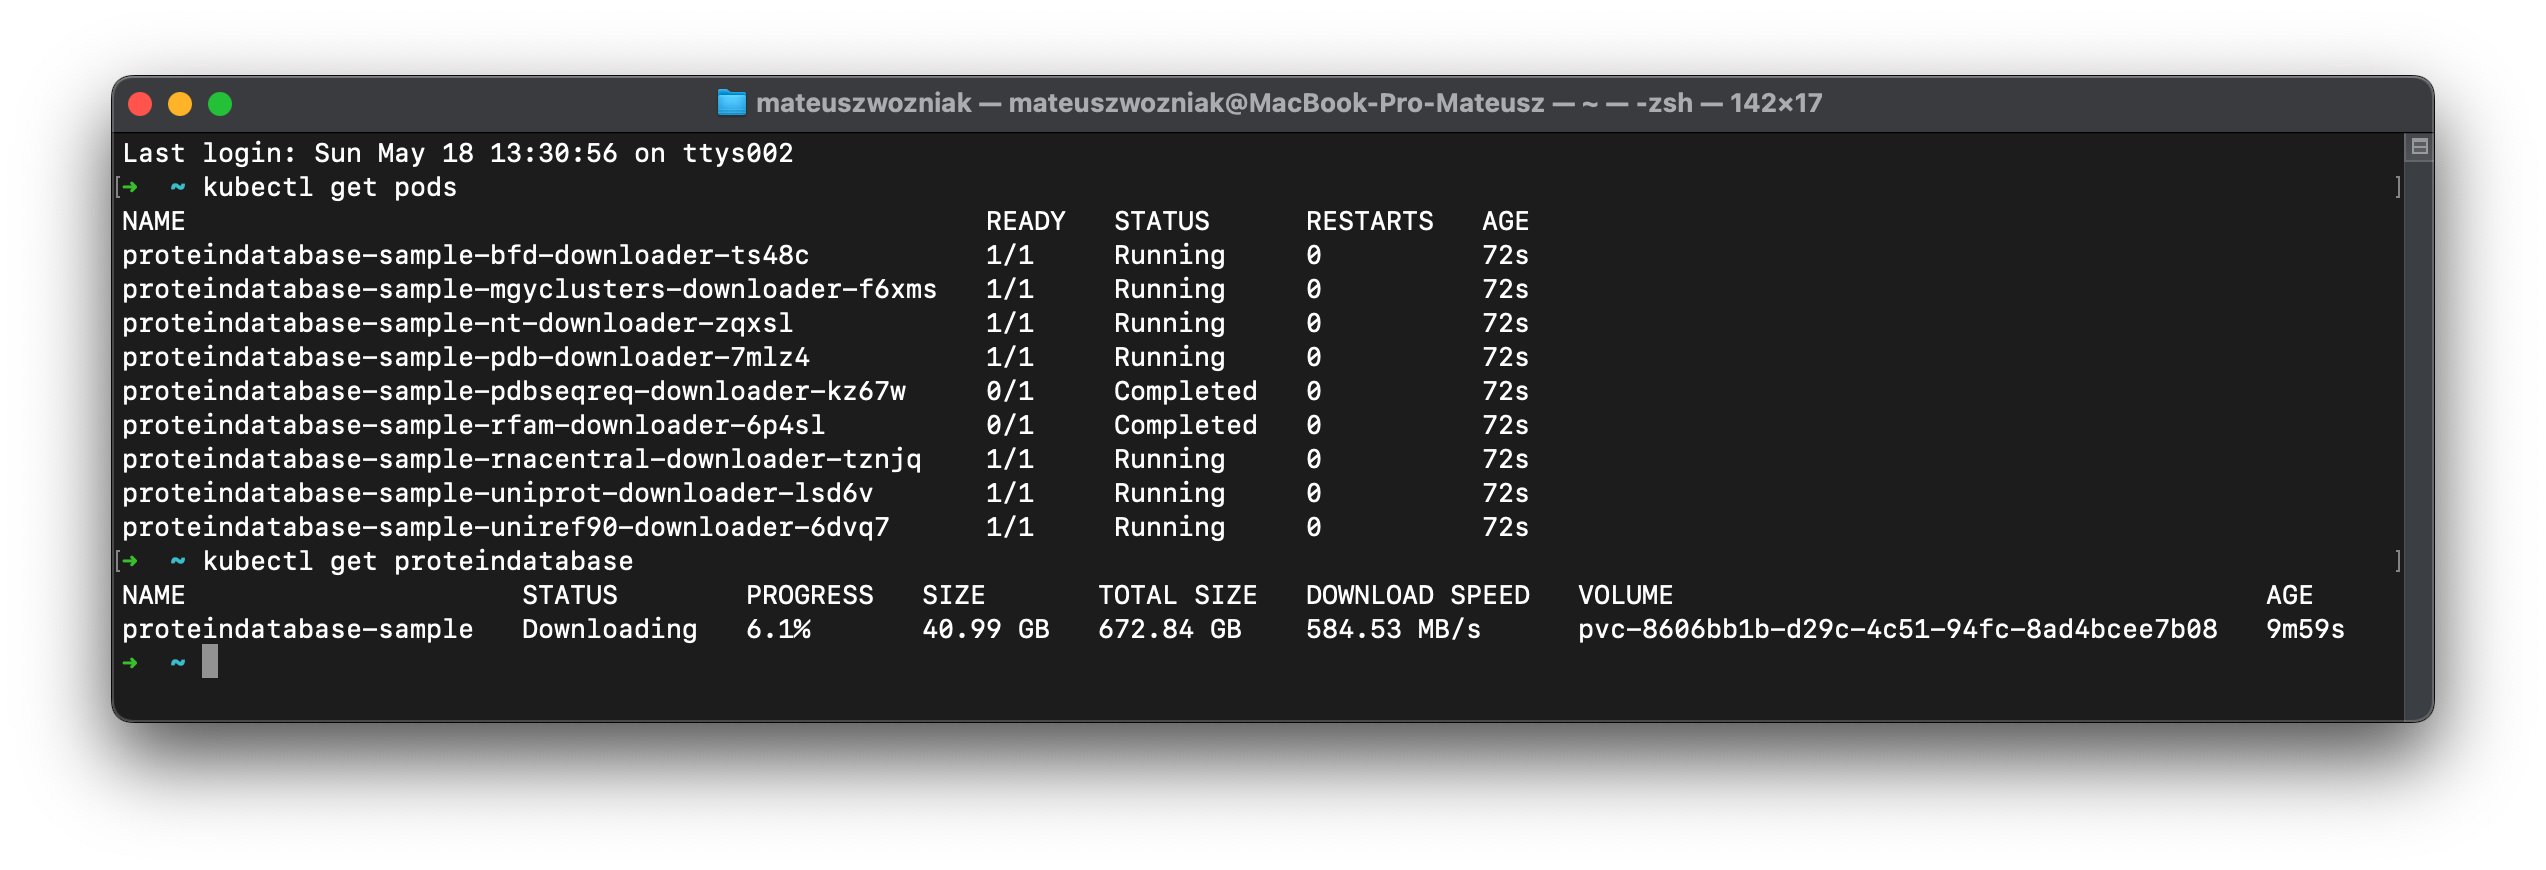
\includegraphics[width=\textwidth]{images/proteindatabase_terminal}
    \caption{Terminal output presenting \texttt{ProteinDatabase} resource}
    \label{fig:proteindatabase_terminal}
\end{figure}

Additionally, KubeFold supports the \texttt{ProteinConformationPrediction} resource definition.
It represents a single protein conformation computation based on a provided amino acid sequence.
An example definition is shown in listing~\ref{lst:protein_conformation_prediction}.
Users can specify task settings such as:
\begin{itemize}
    \item the protein database that the AlphaFold algorithm should use for searching
    \item the amino acid sequence as a string of letters
    \item settings for the volume storing temporary computation files
    \item specification of the AlphaFold model weights source.
    In the example code, the source is set as a remote HTTP server.
    \item target location for artifacts.
    In the current version of KubeFold, only AWS S3 object storage is supported (see~\ref{subsec:amazon-s3-object-storage}).
    \item notification options.
    The example code has a single SMS notification configured for a phone number.
\end{itemize}
Management can be done using \texttt{kubectl} as shown in figure~\ref{fig:proteinconformationprediction_terminal}.

\begin{figure}[htbp]
    \centering
    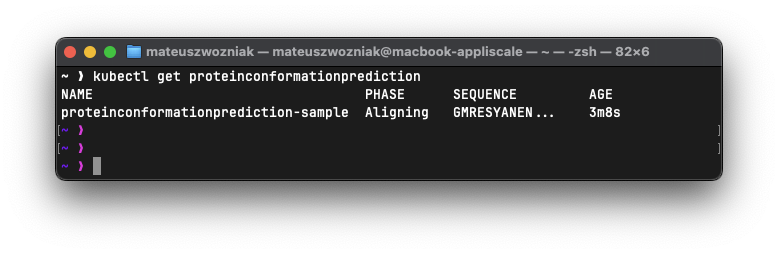
\includegraphics[width=\textwidth]{images/proteinconformationprediction_terminal}
    \caption{Terminal output presenting \texttt{ProteinConformationPrediction} resource}
    \label{fig:proteinconformationprediction_terminal}
\end{figure}

\begin{lstlisting}[language=yaml,caption={Example \texttt{ProteinConformationPrediction} resource definition},label={lst:protein_conformation_prediction}]
apiVersion: data.kubefold.io/v1
kind: ProteinConformationPrediction
metadata:
  name: proteinconformationprediction-sample
spec:
  database: proteindatabase-sample
  protein:
    id: [ 'A','B' ]
    sequence: GMRESY...LQQANDLKQG
  model:
    volume:
      storageClassName: fsx-sc
    weights:
      http: https://staticfilehosting.com/af3.bin.zst
    seeds:
      - 1
  destination:
    s3:
      bucket: kubefold-artifacts-sample
      region: eu-central-1
  notify:
    region: eu-central-1
    sms:
      - "+48140690323"
\end{lstlisting}


\section{Technologies}
All three components were written in Go version 1.24 (more about it in a section~\ref{subsec:go-programming-language}).
This was a natural choice, as Go is the de facto standard for cloud software development.
The source code of the components was archived in the Git repository~\cite{git} on GitHub\cite{github}.

To compile the application and package executable files into a container image, the standard Docker builder was used.

Container images were distributed via the GitHub Container Registry (\textit{ghcr.io})~\cite{ghcr}.
Images were automatically built upon every push tag to Git by the GitHub Actions tool~\cite{github_actions}.
The workflow is shown in figure~\ref{fig:docker-images-flow}.

\begin{figure}[htbp]
    \centering
    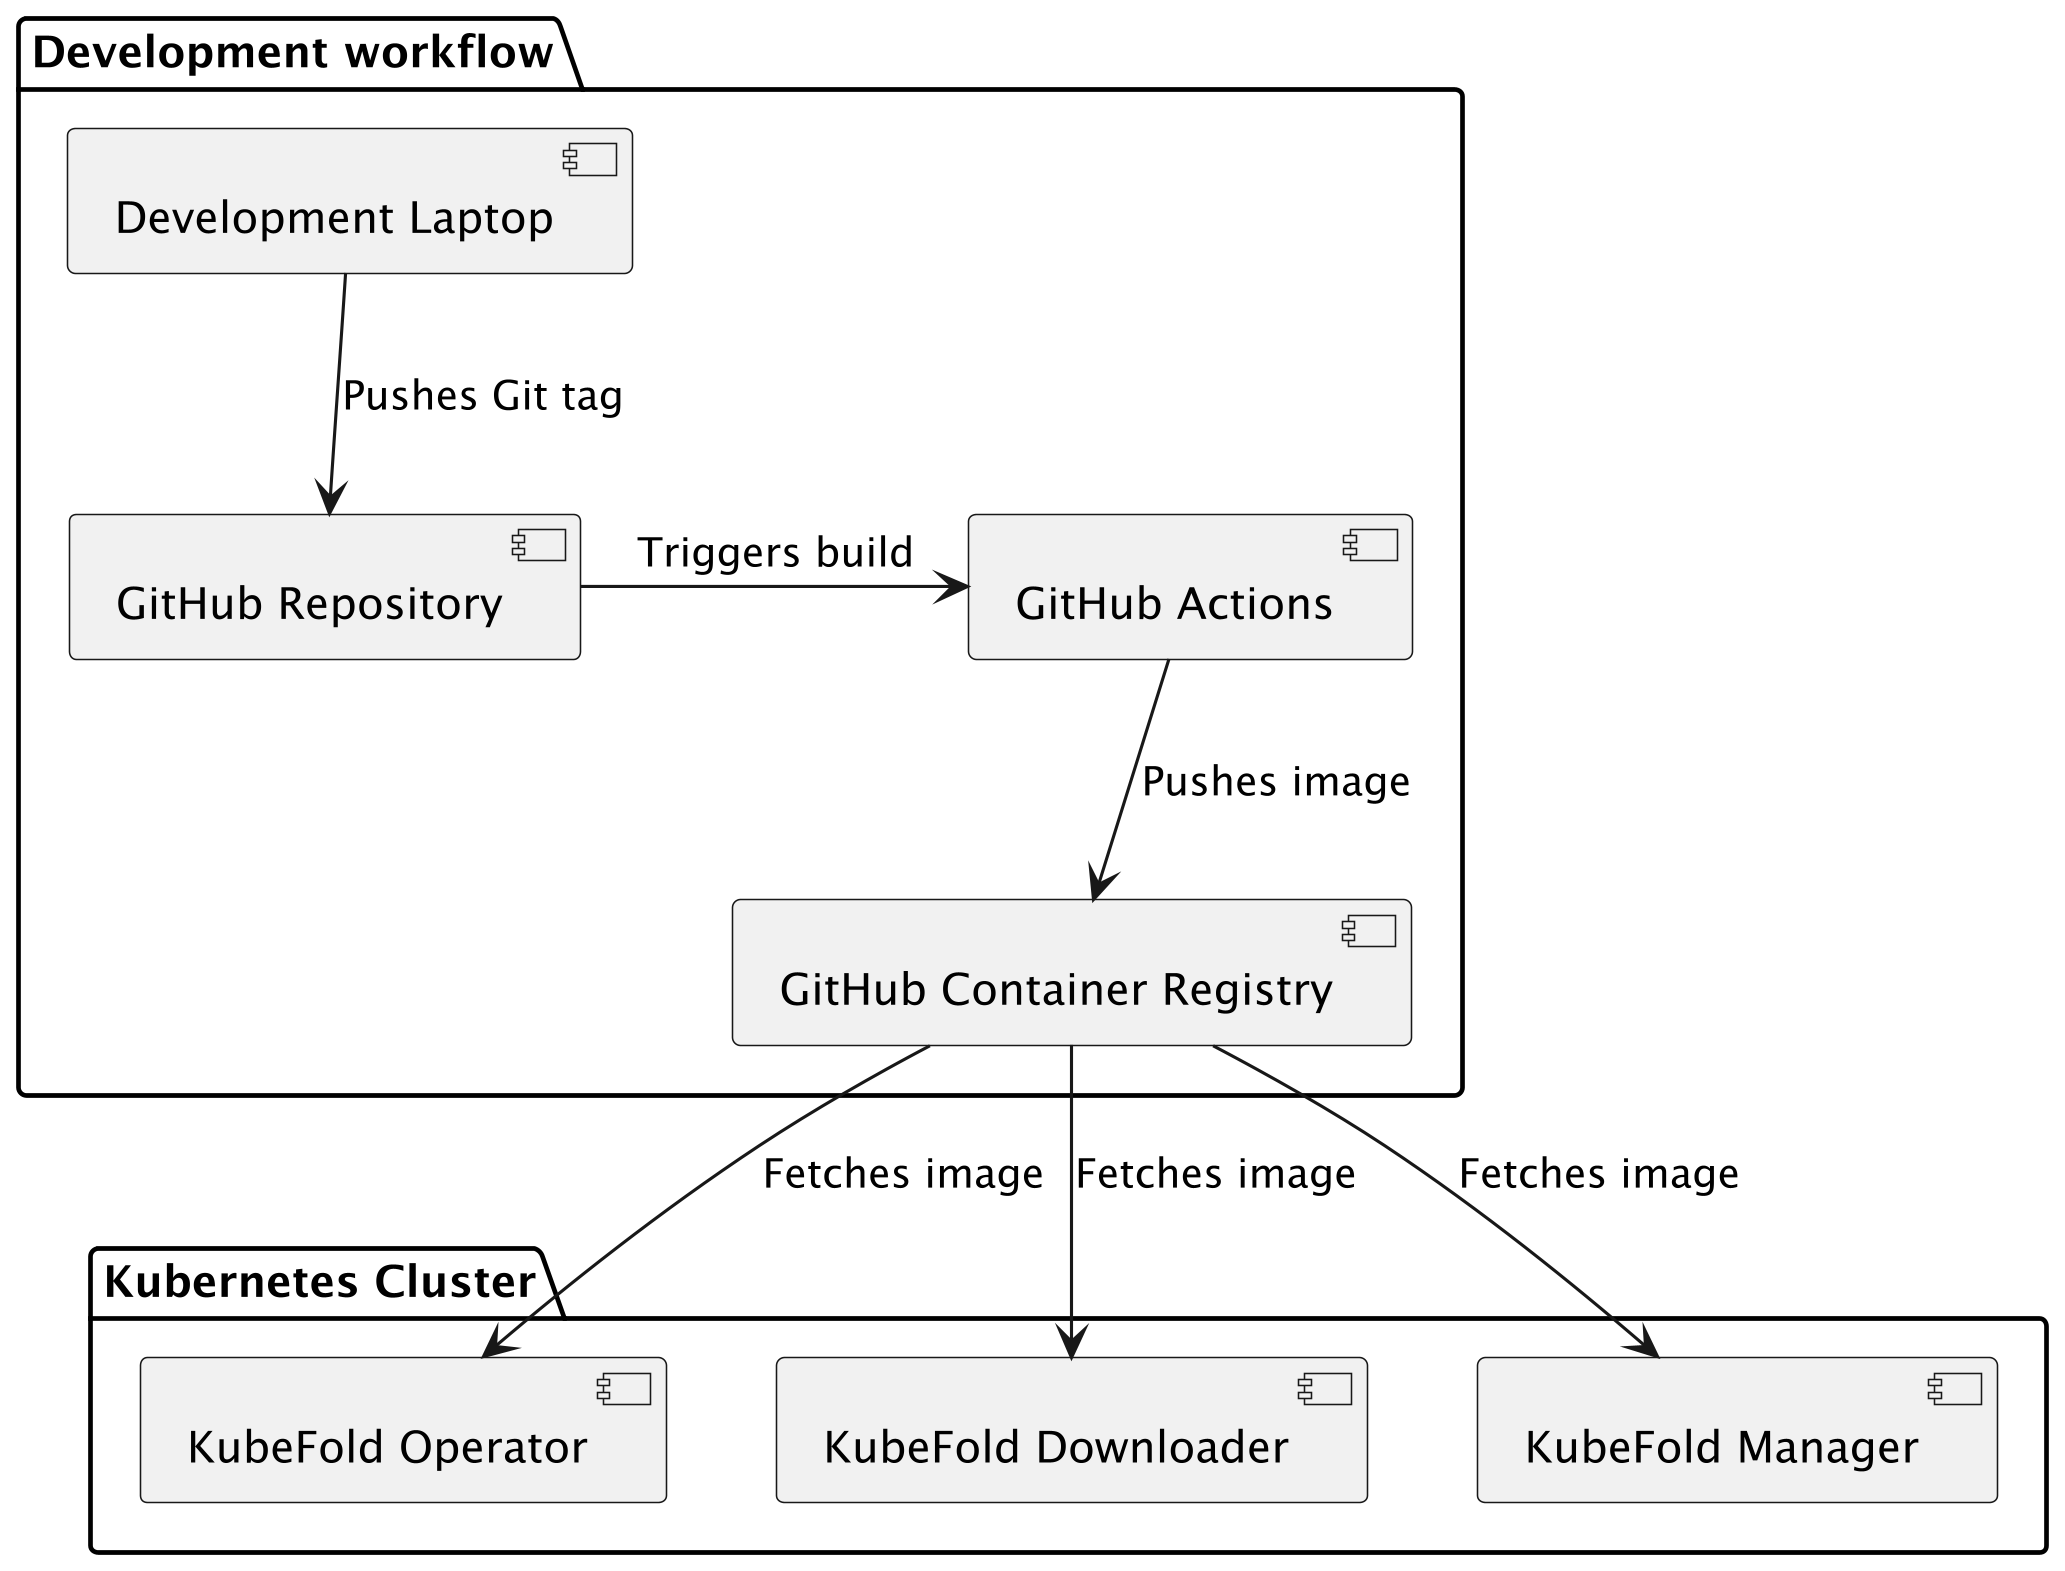
\includegraphics[width=0.8\textwidth]{images/images}
    \caption{Development workflow between GitHub and cluster}
    \label{fig:docker-images-flow}
\end{figure}

The Kubernetes Operator component (described in more detail in~\ref{subsec:component-operator}) was created based on the KubeBuilder framework~\cite{kubebuilder}.
KubeBuilder is a framework that facilitates writing native Kubernetes operators.
It creates project directory structure and immediately provides management of elements such as:
\begin{itemize}
    \item Leader election-some operator instances can run on multiple cluster nodes simultaneously, but if there is a need to select a single distinguished instance, the leader election selects it.
    \item Generation of installation scripts-KubeBuilder has the ability to generate ready-to-use installation scripts that can later be used for automatic operator installation and all its dependencies in the cluster with a single \texttt{kubectl apply} command.
    \item Role and permission definitions.
    Kubernetes uses an authorization model called \textit{RBAC} (Role-Based Access Control)~\cite{k8s_rbac}.
    KubeBuilder checks what permissions an operator instance should have and ensures that the appropriate permissions are granted to it.
\end{itemize}


\section{Architecture}

Both introduced CRD resources manage certain subordinate resources.

The \texttt{ProteinDatabase} resource primarily creates: a persistent volume claim that will store data from protein databases and a set of jobs that correspond to downloading individual databases.
The resource dependency architecture is shown in figure~\ref{fig:proteindatabase}.
The number of jobs is exactly the same as the number of selected databases defined in the YAML code.
Due to this split process of downloading, it is possible for multiple nodes to download independent data at the same time.
In such a case, the total throughput increases, as it will not be limited by the speed of the single node network interface.
All pods created by the jobs connect to a common volume and download databases from Google servers using HTTP protocol.
The progress is logged to the \texttt{stdout} of the container in real time.
This enables the operator to read container logs and monitor progress in real time.
Pods and volume are connected to the \texttt{ProteinDatabase} resource using the \textit{ownerReferences} mechanism.
If the parent resource is deleted, the subordinate resources will also be automatically deleted.
The automatic resource cleanup functionality is handled in the Kubernetes implementation, not in the operator.

\begin{figure}[htbp]
    \centering
    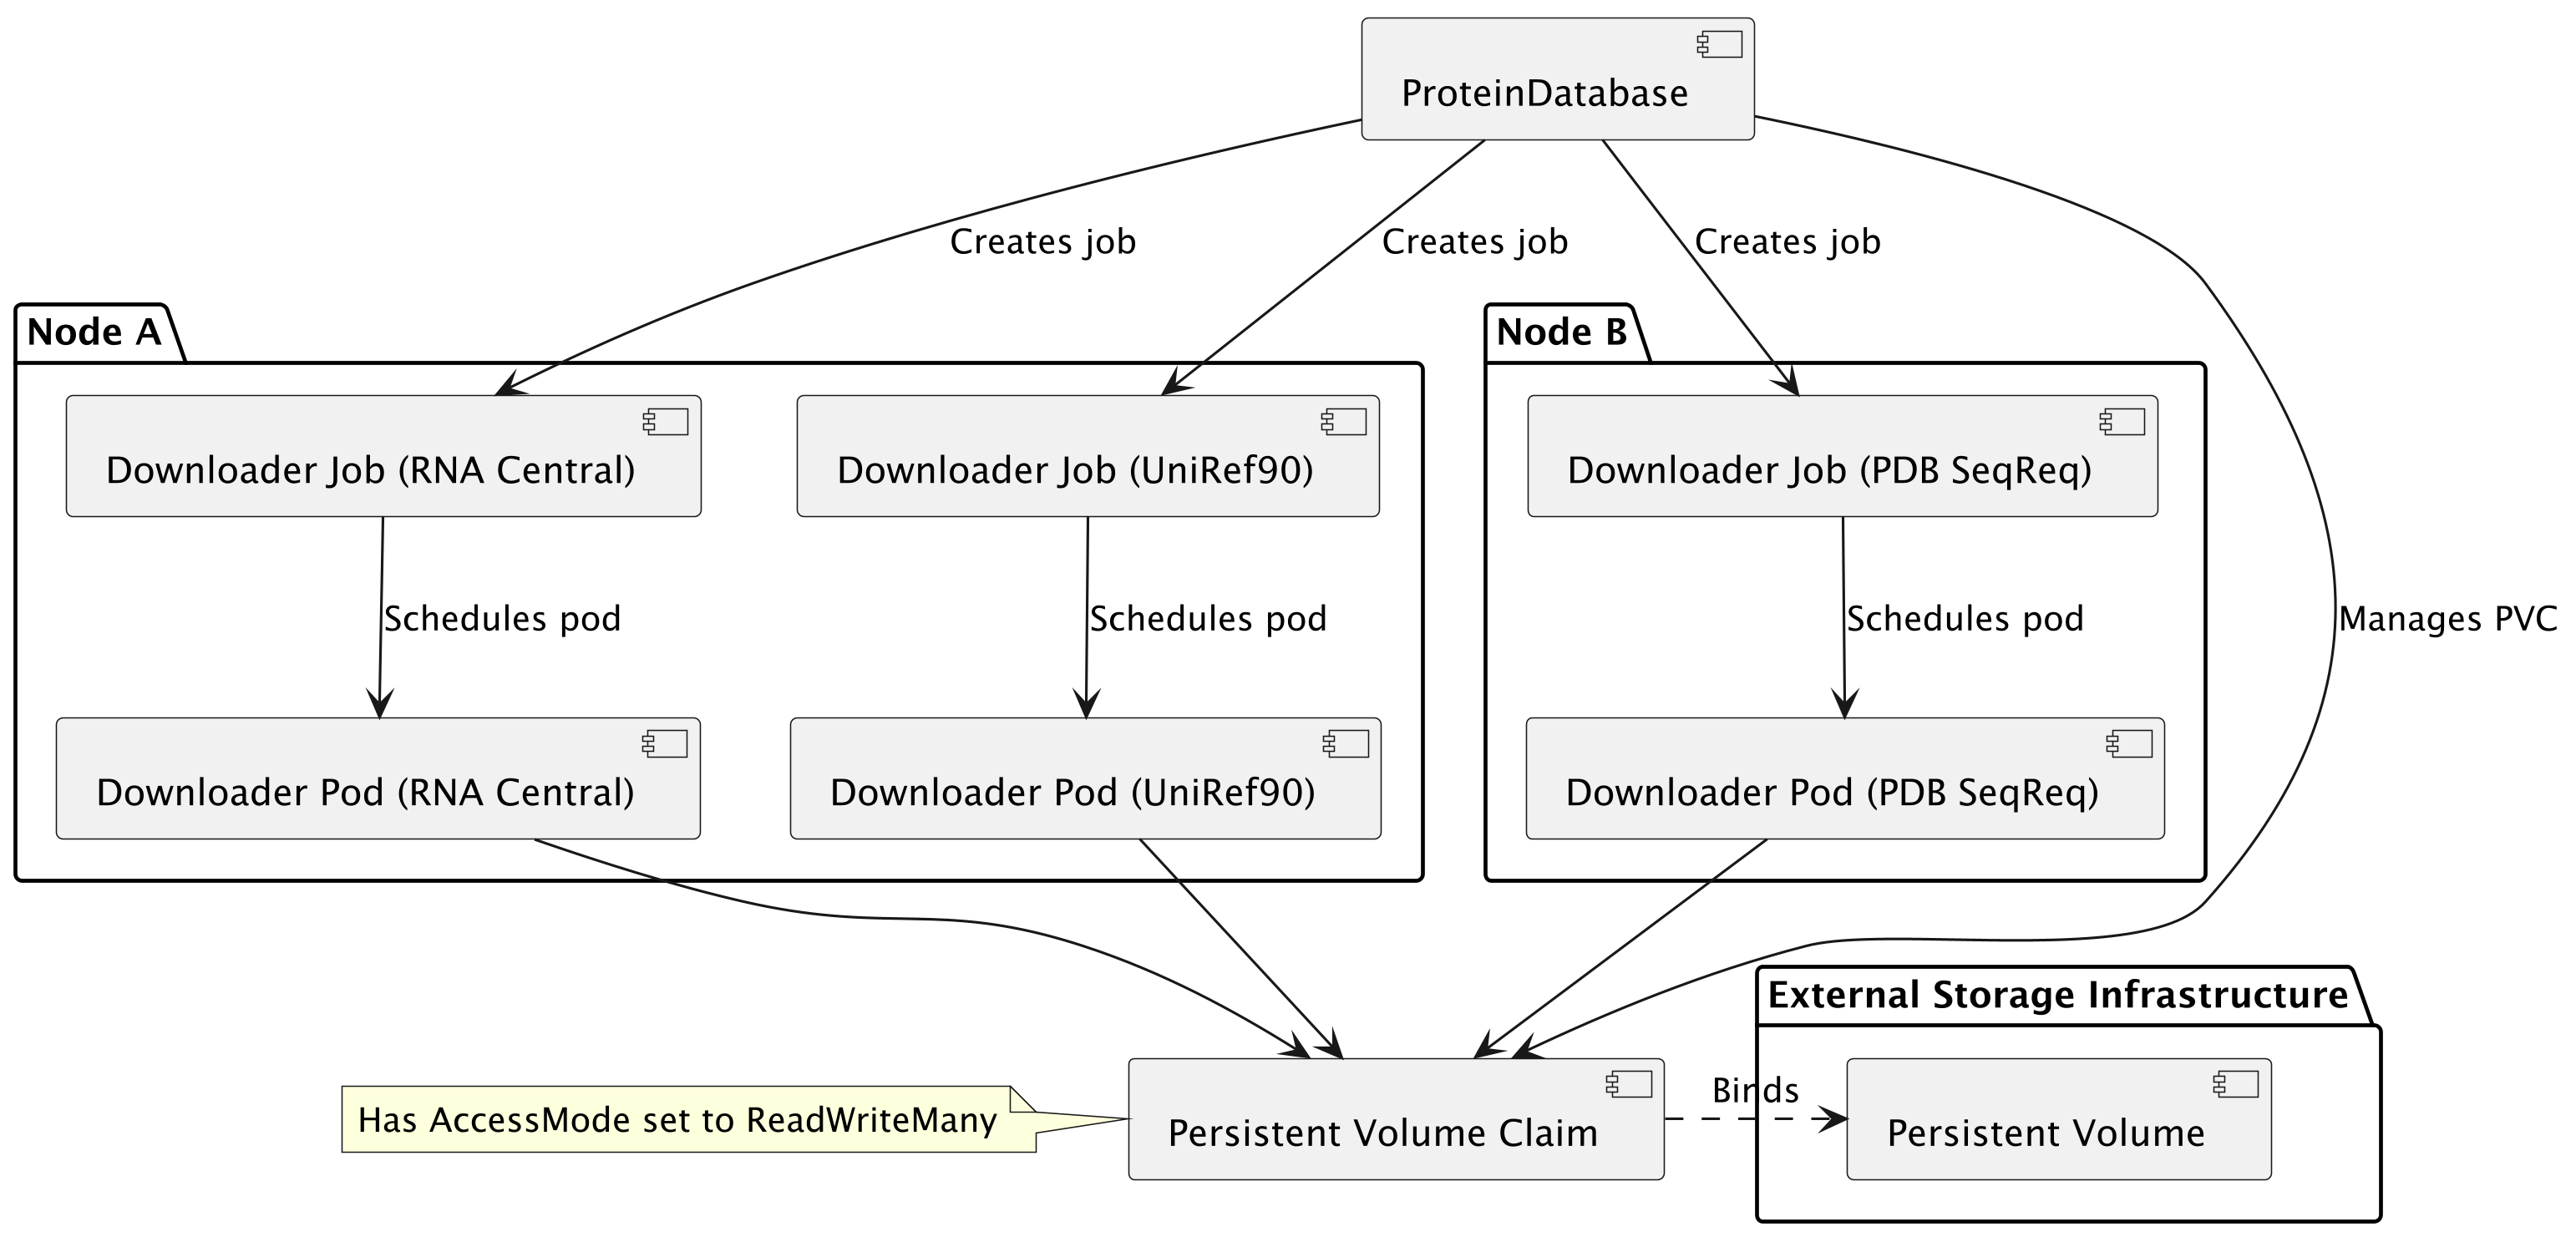
\includegraphics[width=\textwidth]{images/proteindatabase}
    \caption{Cluster resource architecture of ProteinDatabase}
    \label{fig:proteindatabase}
\end{figure}

\begin{figure}[htbp]
    \centering
    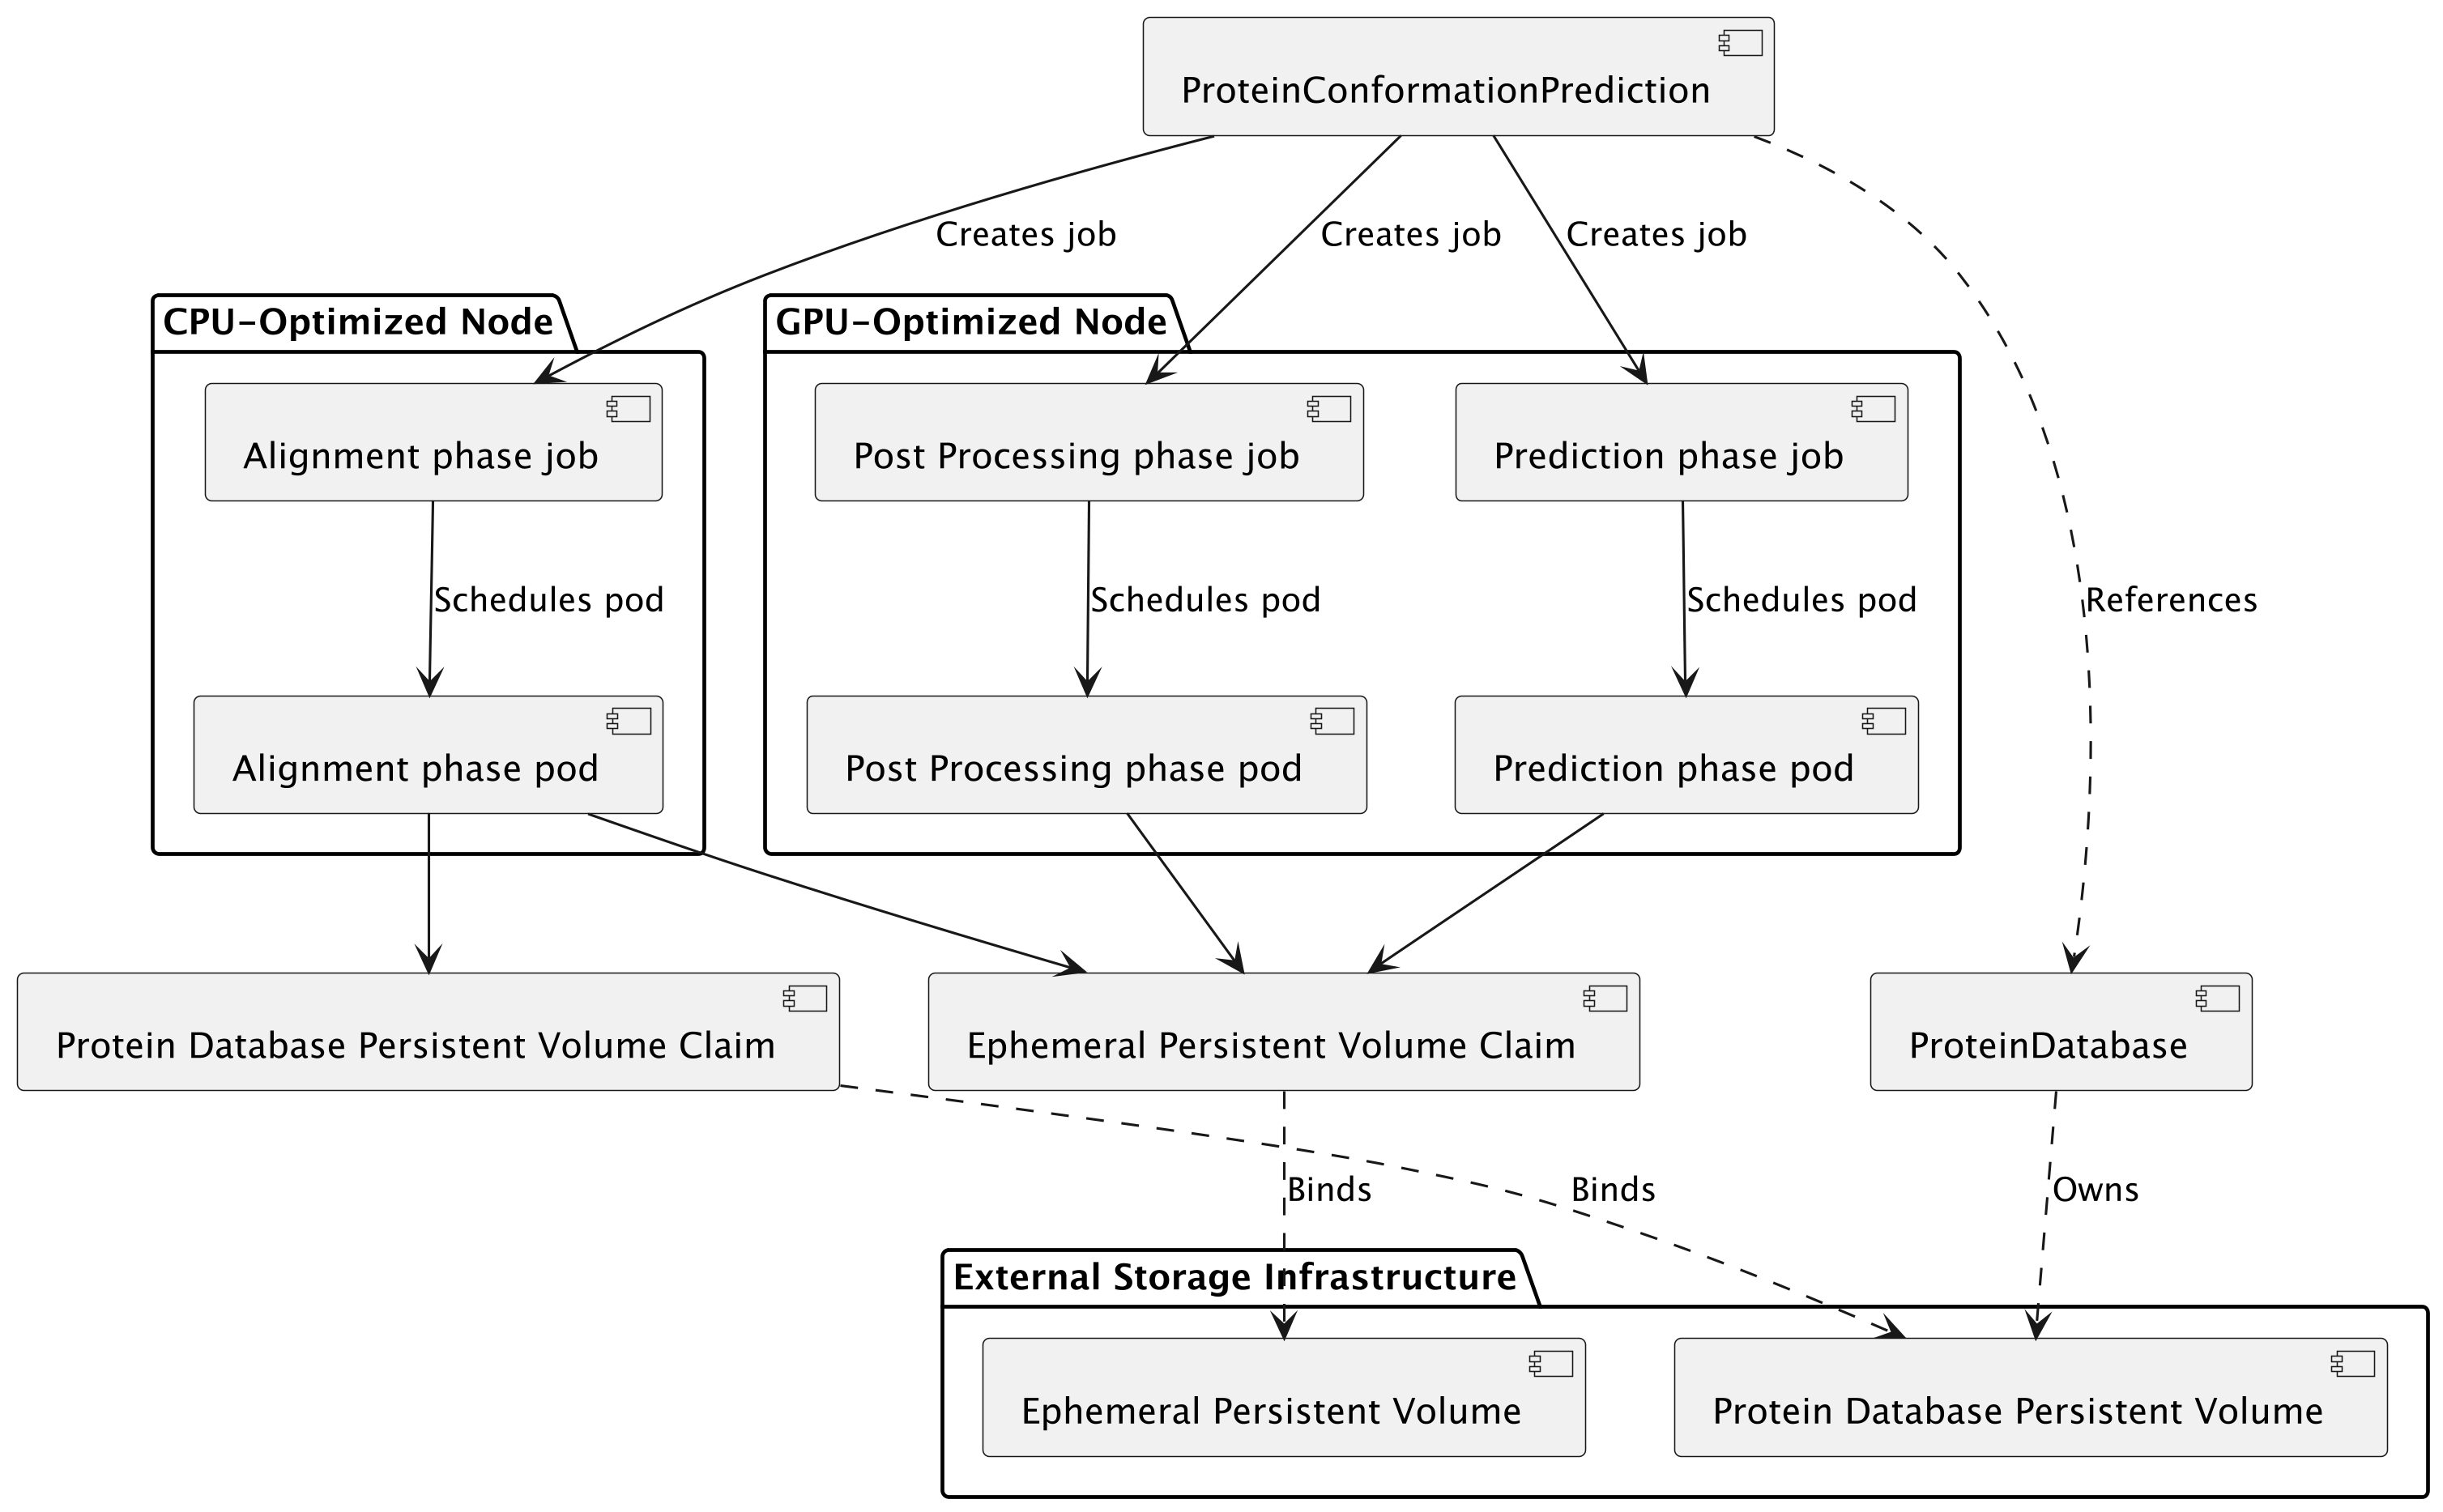
\includegraphics[width=\textwidth]{images/proteinconformationprediction}
    \caption{Cluster resource architecture of ProteinConformationPrediction}
    \label{fig:proteinconformationprediction}
\end{figure}

On the other hand, the \texttt{ProteinConformationPrediction} resource manages three jobs.
\begin{itemize}
    \item Alignment Phase.
    In this phase, AlphaFold searches existing protein databases to find matches.
    This phase takes place on scheduled instances optimized for CPU. The pod uses the AlphaFold image.
    \item Prediction Phase.
    This phase is when the algorithm performs the actual prediction of the three-dimensional structure of the protein.
    In this phase, pods are scheduled on instances equipped with tensor computing accelerators.
    The pod also uses the AlphaFold image.
    \item Post Processing Phase.
    This phase is responsible for sending computation artifacts to the destination data storage and optionally sending notifications to the research team members.
    The pod uses the \textit{manager} component image.
\end{itemize}

Therefore, each \texttt{ProteinConformationPrediction} instance corresponds to exactly three jobs and three pods.
In addition, \texttt{ProteinConformationPrediction} creates a \texttt{PersistentVolumeClaim} for temporary data.
In this volume, artifacts from the Alignment phase and potentially found protein structures are stored.

Similarly to the \texttt{ProteinDatabase} resource, the resources are connected using the \textit{ownerReferences} mechanism.
The resource dependency architecture is shown in figure~\ref{fig:proteinconformationprediction}.


\section{Components Overview}

\subsection{Kubernetes Operator}\label{subsec:component-operator}
\textit{Code repository: \url{https://github.com/kubefold/operator}}

The main component of the KubeFold platform written in Go.
The operator is installed on the Kubernetes cluster as a Deployment resource and connects to the Kubernetes API Server using the appropriate ClusterRole.
This gives it access to the REST API interface, which allows managing resources created within the cluster.

The most important elements of the KubeFold operator are two controllers, responsible for reconciling two CRD definitions introduced within the project.
Each cluster operator works on the infinite control loop, that constantly monitors changes in expected resource states in the cluster and adjusts the actual state to be as close as possible to the specified.
In the case of the KubeFold operator, the control loop works only on a single operator instance.
The election system provided by the KubeBuilder tool determines which running instance will be selected.

The first controller reconciles the \texttt{ProteinDatabase} resource.
In case of a new resource of this type appearing, the following operations are performed:
\begin{enumerate}
    \item Creates a new \textt{PersistentVolumeClaim} and sets the \texttt{storageClassName} parameter.
    \item When the \textt{PersistentVolumeClaim} is bound to a specific volume, it creates several jobs corresponding to downloading individual databases.
    Each pod has a mounted this \textt{PVC}.
    \item Starts a log observer-a separate goroutine constantly monitoring job states, pod states, and reading logs from them.
    Thanks to the logs, it is able to dynamically update the \texttt{ProteinDatabase} status informing the user about the progress of downloading and also monitor the connection throughput.
\end{enumerate}
These operations are shown in figure~\ref{fig:proteindatabase_controller}.

\begin{figure}[htbp]
    \centering
    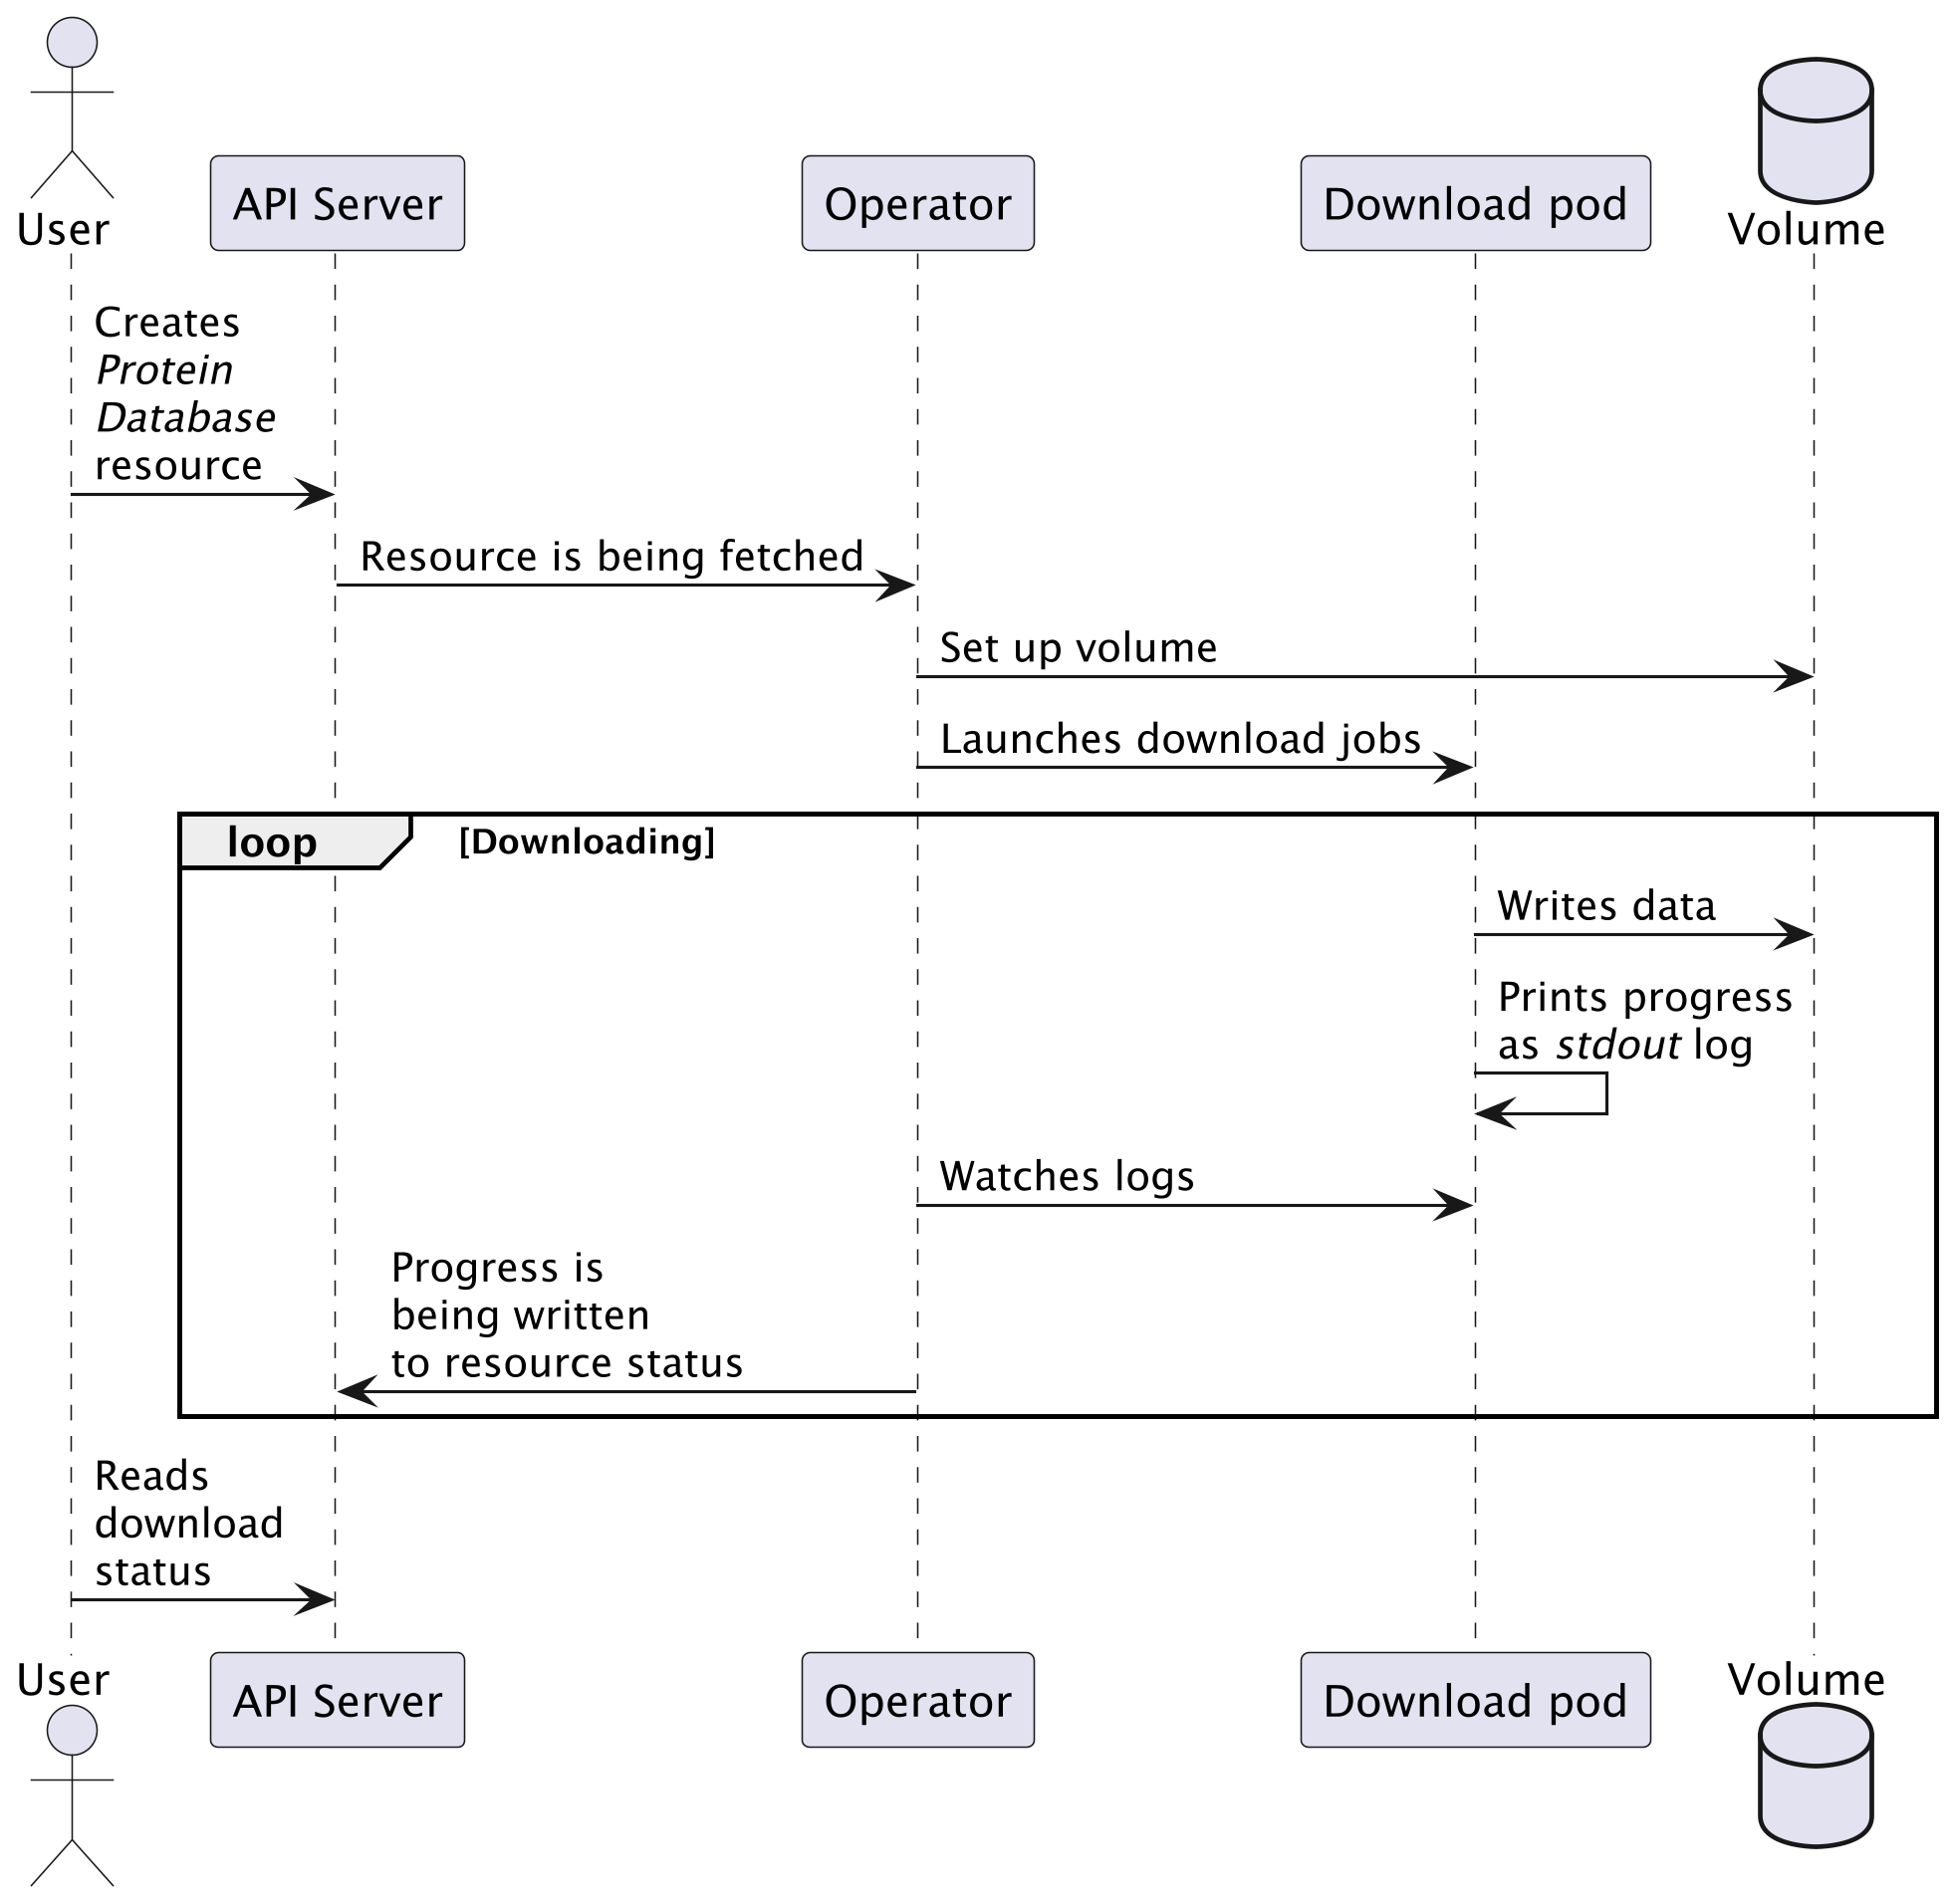
\includegraphics[width=\textwidth]{images/proteindatabase_controller}
    \caption{ProteinDatabase Controller behaviour}
    \label{fig:proteindatabase_controller}
\end{figure}

\begin{figure}[htbp]
    \centering
    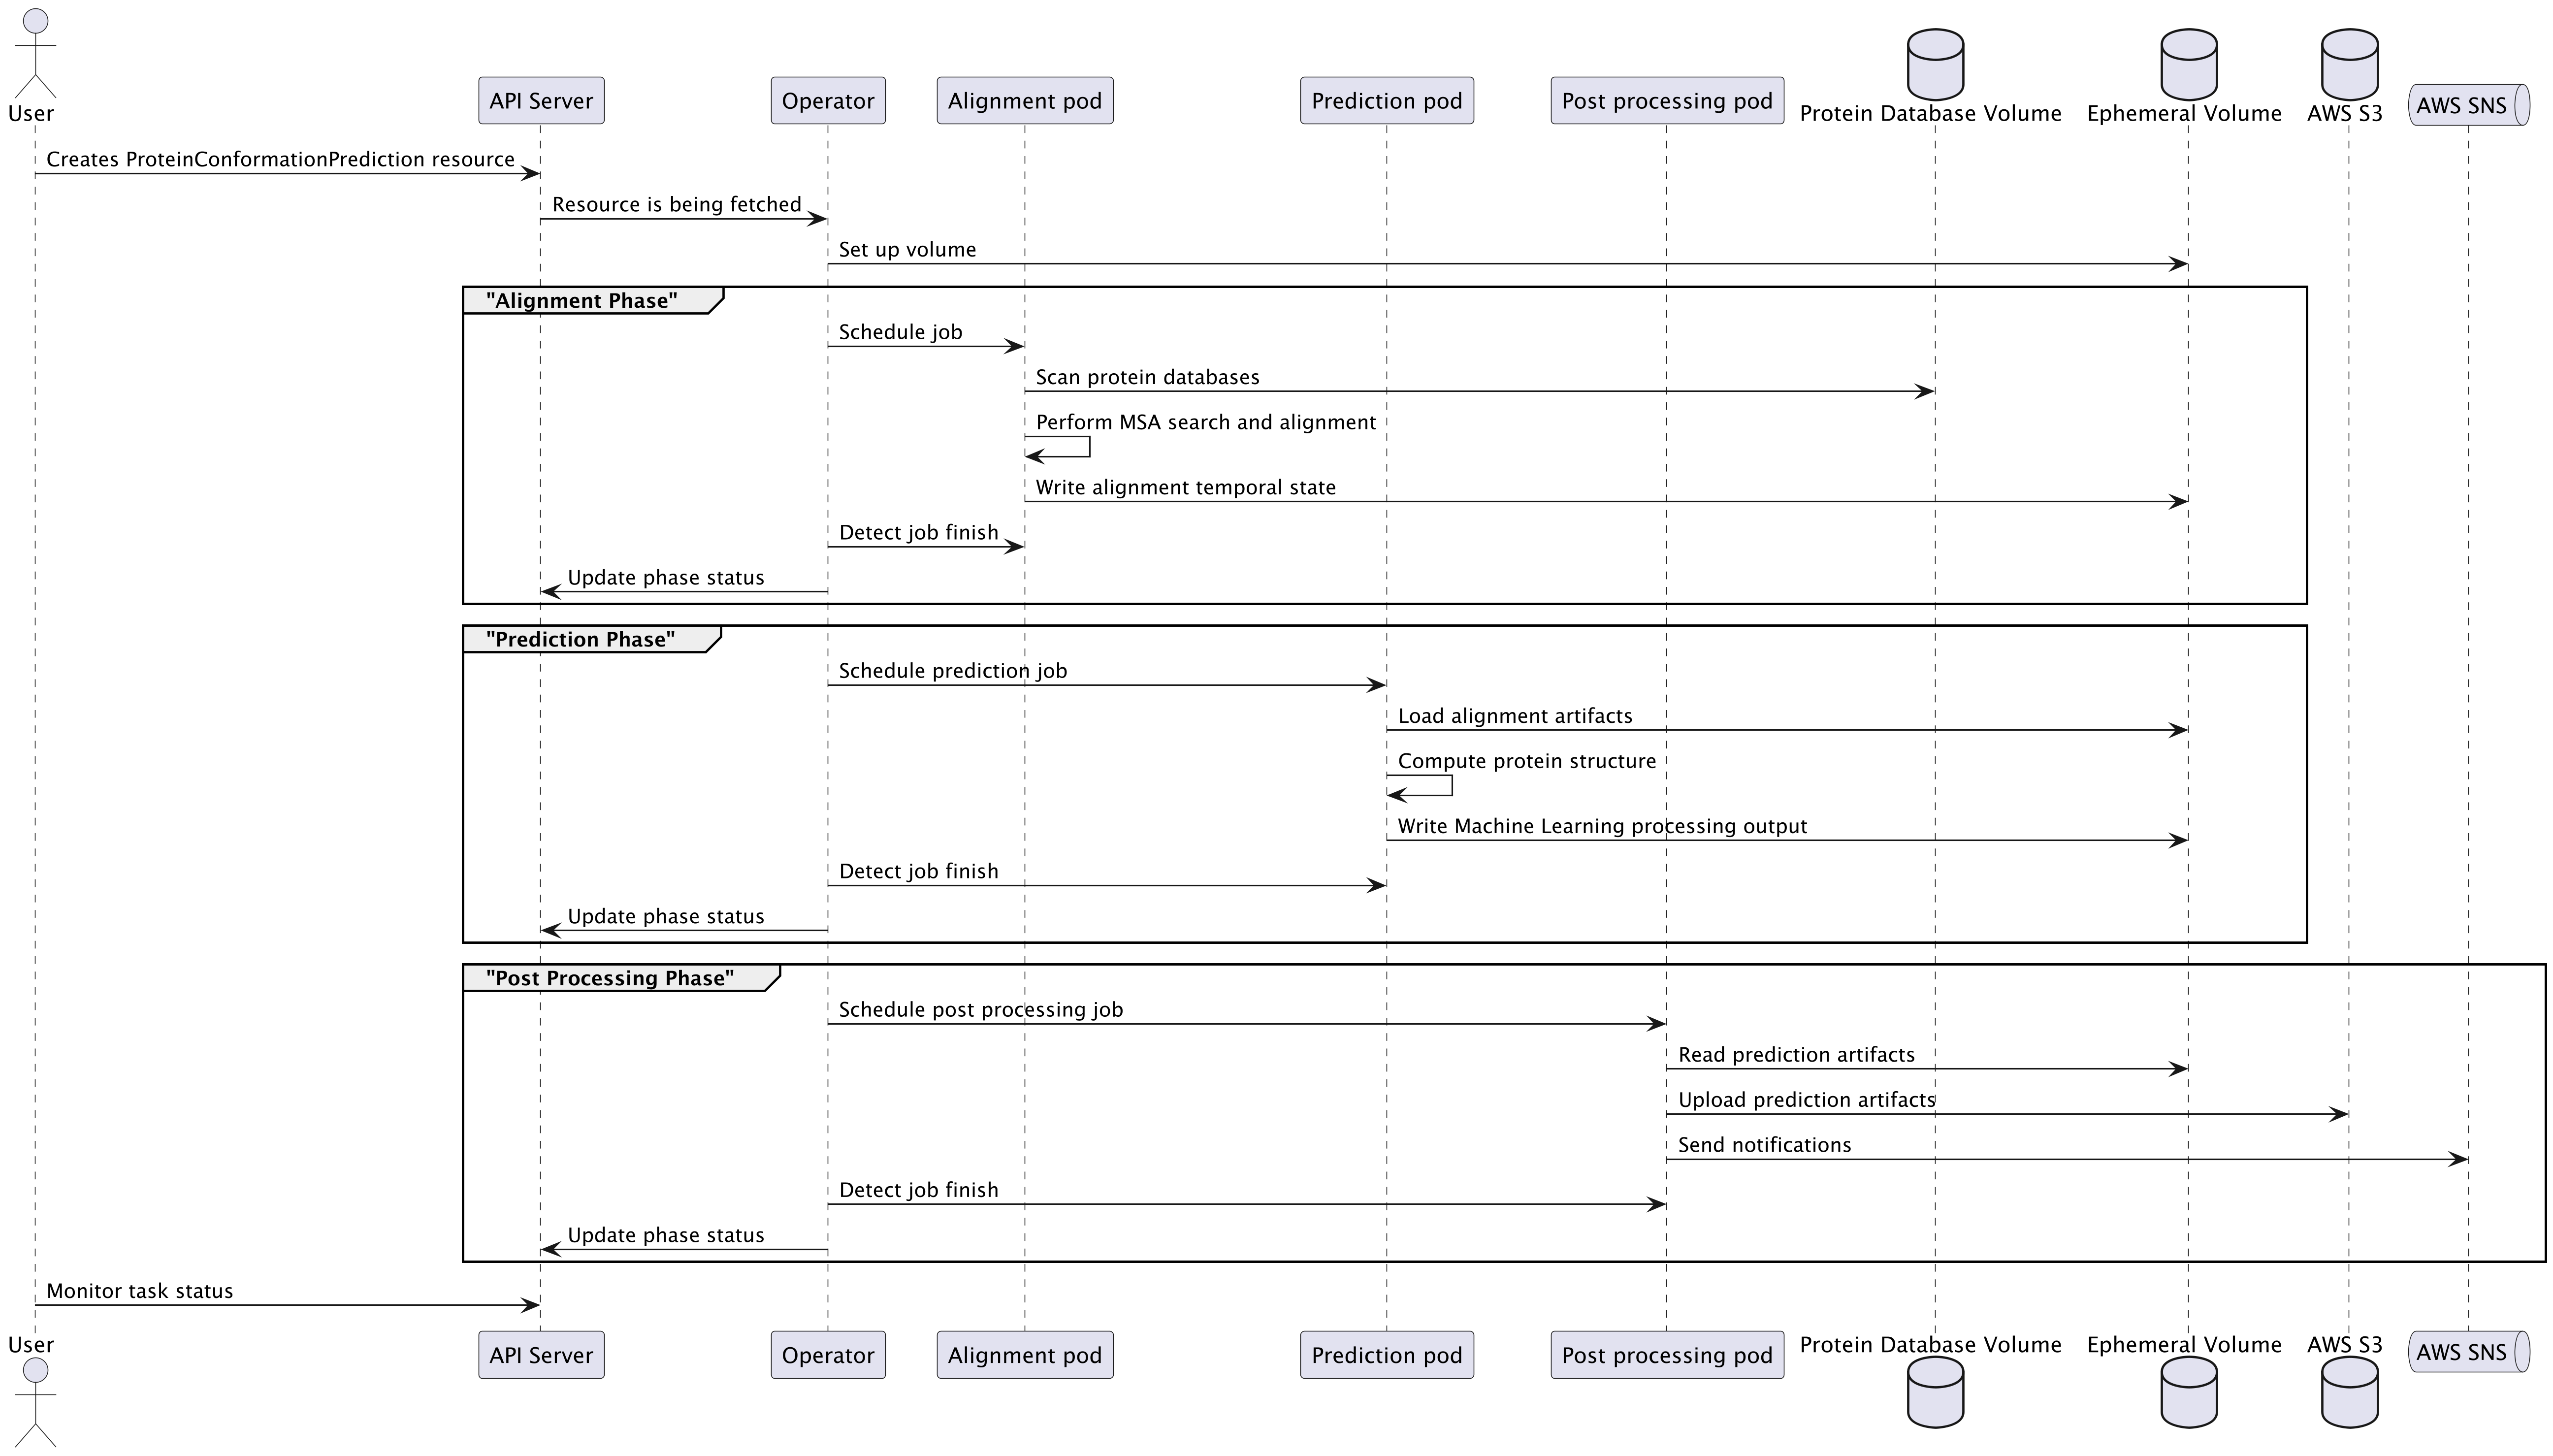
\includegraphics[width=0.9\textwidth]{images/proteinconformationprediction_controller}
    \caption{ProteinConformationPrediction Controller behaviour}
    \label{fig:proteinconformationprediction_controller}
\end{figure}

The second controller handles the \texttt{ProteinConformationPrediction} resource.
It contains the logic responsible for the three prediction phases of the protein structure.
The business logic (shown in figure~\ref{fig:proteinconformationprediction_controller}) after detecting a new resource performs the following steps:
\begin{enumerate}
    \item Creates a new \textit{PersistentVolumeClaim} for storing temporary program AlphaFold files.
    \item Starts a \textit{Job} that performs Alignment of the sequence and saves the state to the temporary volume.
    Also mounts the volume containing the protein databases.
    The AlphaFold program expects initial settings (for example sequence amino acids) as a JSON file named \texttt{fold\_input.json}.
    This file is created in this step using a special \textit{initContainer} ~\cite{k8s_init_containers}.
    The file content is prepared in the operator, then it is encoded to \texttt{base64} and injected into the init container via environment variables.
    The init container uses the \textit{manager} component image (described in~\ref{subsec:component-manager}).
    \item Starts a \textit{Job} corresponding to predicting the three-dimensional structure of the protein.
    The controller mounts the previously used volume, which contains the state from the alignment phase.
    This \textit{Job} has \textit{nodeAffinity} set so it can be scheduled on high-performance GPU nodes.
    \item Starts a \textit{Job} for post processing.
    This step loads computation artifacts and sends them to AWS S3. It also handles queuing notifications (e.g.
    SMS) for individual research team members.
\end{enumerate}

\subsection{Downloader Component}\label{subsec:component-downloader}
\textit{Code repository: \url{https://github.com/kubefold/downloader}}

The \textit{downloader} component is responsible for downloading a single selected protein database.
Running this component in a container automatically starts download process.
The container expects the following environment variables to be configured:

\begin{itemize}
    \item \texttt{DATASET} - the name of the dataset.
    The acceptable values of this variable are predefined.
    They are:
    \subitem \texttt{mgy\_clusters\_2022\_05.fa} - MGY Clusters
    \subitem \texttt{bfd-first\_non\_consensus\_sequences.fasta} - BFD non-consensus sequences
    \subitem \texttt{uniref90\_2022\_05.fa} - UniRef90
    \subitem \texttt{uniprot\_all\_2021\_04.fa} - UniProt
    \subitem \texttt{pdb\_2022\_09\_28\_mmcif\_files.tar} - PDB mmCIF files
    \subitem \texttt{pdb\_seqres\_2022\_09\_28.fasta} - PDB sequence resources
    \subitem \texttt{rnacentral\_active\_seq\_id\_90\_cov\_80\_linclust.fasta} - RNACentral
    \subitem \texttt{nt\_rna\_2023\_02\_23\_clust\_seq\_id\_90\_cov\_80\_rep\_seq.fasta} - NT RNA
    \subitem \texttt{rfam\_14\_9\_clust\_seq\_id\_90\_cov\_80\_rep\_seq.fasta} - RFam
    \item \texttt{DESTINATION} - the path to the output directory.
    \item \texttt{RATE} (optional) - the download speed limit expressed in kilobytes per second.
    The default process download does not have an upper limit set.
\end{itemize}.

All databases are hosted in the Google Cloud Storage service.
Almost all of them are \textit{.fasta}~\cite{pearson1988fasta} files compressed with the \textit{ZStandard} (or shorter \textit{zstd}) algorithm from Facebook~\cite{zstandard}.
The exception is the \texttt{pdb\_2022\_09\_28\_mmcif\_files.tar} file, which is a TAR archive (also compressed with \textit{zstd}).

The component downloads and decompresses files at the same time.
Every few moments, a separate goroutine monitors the progress of already downloaded data and outputs to \texttt{stdout} a logline with the current state.
A sample logline is shown in listing~\ref{lst:downloader_logline}.
Thanks to this, the operator can read download progress and update the \texttt{ProteinDatabase} status.
After successful completion or interrupted download, the process exits logging the valid message to logs and returning the appropriate exit code.

\begin{lstlisting}[language=txt,caption={Sample logline from downloader},label={lst:downloader_logline}]
{"dataset":"rnacentral_active_seq_id_90_cov_80_linclust.fasta","level":"info","msg":"Download progress","size":7700349721,"time":"2025-05-17T16:53:52+02:00","total":13860314914,"type":"download","unit":"bytes"}
\end{lstlisting}

\subsection{Manager Component}\label{subsec:component-manager}
\textit{Code repository: \url{https://github.com/kubefold/manager}}

The \textit{manager} component is responsible for three independent tasks:
\begin{itemize}
    \item configuring the \textt{fold\_input.json} file for the AlphaFold program.
    \item sending computation artifacts to the AWS S3 service (more about it in section~\ref{subsec:amazon-s3-object-storage}).
    \item queuing notifications using the AWS SNS / AWS End User Messaging service (more about it in section~\ref{subsec:amazon-sns})
\end{itemize}

The selected operation depends on which environment variables are configured in the container.
For each operation, two environment variables are mandatory:
\begin{itemize}
    \item \texttt{INPUT\_PATH} - the path to the AlphaFold data input directory
    \item \texttt{OUTPUT\_PATH} - the path to the AlphaFold data output directory
\end{itemize}

To save the \textt{fold\_input.json} file, the \texttt{ENCODED\_INPUT} variable should be set, which should contain the encoded in \texttt{base64} JSON configuration.

To send artifacts, the \texttt{BUCKET} environment variable should be set to the S3 bucket path (full URL, including \textt{s3:\/\/}).
To send a notification using the AWS End User Messaging service, the container must have the \texttt{NOTIFICATION\_PHONES} and \texttt{NOTIFICATION\_MESSAGE} variables set.
The variable with phone numbers can contain more than one recipient-in such a case, phone numbers should be provided as a comma-separated list.

If using AWS services, the AWS client variables should be configured.
This can be done using environment variables such as \texttt{AWS\_ACCESS\_KEY\_ID} and \texttt{AWS\_SECRET\_ACCESS\_KEY}.
An alternative is to configure the AWS IAM role to be used by the container and have access permissions to the individual services.